% =====================================================================
%   EAST DELTA UNIVERSITY  --  B.Sc. THESIS TEMPLATE
%   Department of Computer Science & Engineering
% ---------------------------------------------------------------------
%   HOW TO USE (for students who are new to LaTeX)
%   1. Upload this file and the three image files into ONE Overleaf
%      project (no folders needed):
%         main.tex, references.bib,
%         edu_logo.jpg, edu_logo_inner.png, sample_figure.png
%   2. Fill in STEP 1 below (your name, ID, title ...). These details are
%      then printed automatically on every page that needs them.
%   3. Scroll down to the part you are writing (search for "CHAPTER 1",
%      "ABSTRACT", etc.) and replace the sample text.
%   4. Text in RED is guidance. Delete the whole \guidance{...} line when
%      you no longer need it.
%   5. Press "Recompile". If the Table of Contents looks wrong, press
%      Recompile once more.
%
%   You do NOT need to edit anything inside the box marked
%   "LAYOUT SETTINGS -- DO NOT EDIT". Those lines reproduce the official
%   Word template (page size, fonts, spacing).
% =====================================================================

\documentclass[12pt]{report}

% =====================================================================
%   STEP 1 -- YOUR DETAILS  (edit the text inside the last { } only)
% =====================================================================
\newcommand{\ThesisTitle}{[ENTER COMPLETE TITLE OF THE THESIS]}
\newcommand{\StudentName}{[TYPE STUDENT'S NAME]}
\newcommand{\StudentID}{[TYPE STUDENT'S ID]}
\newcommand{\SupervisorName}{[TYPE INSTRUCTOR'S NAME]}
\newcommand{\SupervisorDesignation}{[TYPE DESIGNATION]}
\newcommand{\SubmissionMonthYear}{[Month and Year]}
\newcommand{\DeclarationDate}{[Enter Date]}
% Board of Examiners (the Supervisor is taken from the lines above)
\newcommand{\ChairmanName}{Faculty Name -1}
\newcommand{\ChairmanDesignation}{Associate Dean \& Professor}
\newcommand{\ReviewerName}{Faculty Name -2}
\newcommand{\ReviewerDesignation}{Assistant Professor}
% =====================================================================


% ######################################################################
% #                 LAYOUT SETTINGS -- DO NOT EDIT                      #
% ######################################################################

% ---- Page: US Letter, Left 1.5in, Right/Top/Bottom 1in (as in .docx)
\usepackage[letterpaper,left=1.5in,right=1in,top=1in,bottom=1in,
            footskip=0.45in]{geometry}

% ---- Font: Times New Roman (text and maths)
\usepackage[T1]{fontenc}
\usepackage{mathptmx}
\usepackage{courier}          % typewriter font for \texttt

% ---- Other packages
\usepackage{setspace}
\usepackage{graphicx}
\usepackage{amsmath,amssymb}
\usepackage{float}            % allows [H] = "put the figure exactly here"
\usepackage{array}
\usepackage{xcolor}
\usepackage{enumitem}
\usepackage{titlesec}
\usepackage{tocbibind}        % puts TOC, Lists and References in the TOC
\usepackage[titles]{tocloft}
\usepackage[font=bf,labelsep=quad]{caption}
\usepackage[hidelinks]{hyperref}
\usepackage{etoolbox}

% ---- line spacing ------------------------------------
% Word's "Multiple" spacing for Times New Roman = m x 1.149 x font size.
% \WordFont{size}{multiple} gives exactly that, so the numbers written
% in this file are the SAME numbers you see in Word's Paragraph dialog.
\newcommand{\WordFont}[2]{%
  \def\baselinestretch{1}\fontsize{#1}{\fpeval{#1*1.149*#2}}\selectfont}
% \WordSpacing{multiple} sets the spacing for 12 pt running text.
\newcommand{\WordSpacing}[1]{\setstretch{\fpeval{#1*1.149*12/14.5}}}

% ---- Body text: TNR 12 pt, double spacing (Word 2.0), justified,
%      10 pt after each paragraph, no first-line indent
\WordSpacing{2.0}
\setlength{\parindent}{0pt}
\setlength{\parskip}{10pt}

% ---- Helpers
\newcommand{\guidance}[1]{\textcolor{red}{#1}}   % red guidance text
\newcommand{\HeadingAlign}{\centering}           % used by \chapter*

% ---- Chapter heading: "CHAPTER n" / TITLE, TNR 16 bold, centred,
%      Word: Heading 1, 24 pt before, line spacing 3.0
\titleformat{\chapter}[display]
  {\centering\bfseries\WordFont{16}{1.0}}
  {CHAPTER \thechapter}
  {37pt}                        % CHAPTER n -> title (Word 3.0 spacing)
  {}
\titlespacing*{\chapter}{0pt}{50pt}{24pt}

% ---- Un-numbered headings (Declaration, ABSTRACT, ...): TNR 16 bold
%      Word: Heading 1, 24 pt before, line spacing 1.5
\titleformat{name=\chapter,numberless}[block]
  {\HeadingAlign\bfseries\WordFont{16}{1.0}}{}{0pt}{}
\titlespacing*{name=\chapter,numberless}{0pt}{33pt}{24pt}

% ---- Section (1.1): TNR 14 bold  |  Sub-section (1.1.1): TNR 13 bold
\titleformat{\section}{\bfseries\WordFont{14}{1.0}}{\thesection}{1em}{}
\titlespacing*{\section}{0pt}{18pt}{6pt}
\titleformat{\subsection}{\bfseries\WordFont{13}{1.0}}{\thesubsection}{1em}{}
\titlespacing*{\subsection}{0pt}{14pt}{4pt}

% ---- Page numbers: centred at the bottom
\pagestyle{plain}

% ---- Captions: TNR 9 pt bold, "Figure 4.1  TEM Image"
\DeclareCaptionFont{nine}{\WordFont{9}{1.0}}
\captionsetup{font={bf,nine},labelfont={bf,nine},labelsep=quad}
\captionsetup[table]{position=above,skip=6pt}
\captionsetup[figure]{position=below,skip=6pt}

% ---- Heading names (same wording/case as the Word template)
\renewcommand{\contentsname}{TABLE OF CONTENTS}
\renewcommand{\listtablename}{LIST OF TABLES}
\renewcommand{\listfigurename}{LIST OF FIGURES}
\renewcommand{\bibname}{References}

% ---- Table of contents (as in the Word template): all entries bold,
%      no dot leaders, chapters 12 pt, sections 10 pt, no indentation,
%      section numbers in a 0.67 in column, 5 pt after each entry
\renewcommand{\cftchapfont}{\bfseries\WordFont{12}{1.15}}
\renewcommand{\cftchappagefont}{\bfseries\WordFont{12}{1.15}}
\renewcommand{\cftchappresnum}{CHAPTER~}
\renewcommand{\cftchapaftersnum}{~}
\setlength{\cftchapnumwidth}{1.15in}
\renewcommand{\cftchapleader}{\hfill}
\renewcommand{\cftsecfont}{\bfseries\WordFont{10}{1.15}}
\renewcommand{\cftsecpagefont}{\bfseries\WordFont{10}{1.15}}
\renewcommand{\cftsecleader}{\hfill}
\renewcommand{\cftsubsecfont}{\bfseries\WordFont{10}{1.15}}
\renewcommand{\cftsubsecpagefont}{\bfseries\WordFont{10}{1.15}}
\renewcommand{\cftsubsecleader}{\hfill}
\setlength{\cftchapindent}{0pt}
\setlength{\cftsecindent}{0pt}
\setlength{\cftsubsecindent}{0pt}
\setlength{\cftsecnumwidth}{0.67in}
\setlength{\cftsubsecnumwidth}{0.67in}
\setlength{\cftbeforechapskip}{5pt}
\setlength{\cftbeforesecskip}{5pt}
\setlength{\cftbeforesubsecskip}{5pt}
% List of Tables / Figures: "Table 4.1  Title ...... page"
\renewcommand{\cfttabpresnum}{Table~}
\renewcommand{\cftfigpresnum}{Figure~}
\setlength{\cfttabnumwidth}{0.9in}
\setlength{\cftfignumwidth}{0.95in}
\setlength{\cfttabindent}{0pt}
\setlength{\cftfigindent}{0pt}
\renewcommand{\cfttableader}{\hfill}
\renewcommand{\cftfigleader}{\hfill}

% ---- References (BibTeX): IEEE style, 1.5 spacing, 6 pt between entries.
%      \BibIntro is printed under the "References" heading.
\newcommand{\BibIntro}{}
\patchcmd{\thebibitemlist}{\list}{\BibIntro\list}{}{}
\patchcmd{\thebibitemlist}{\sloppy}{\setlength{\itemsep}{6pt}\sloppy}{}{}

% ---- Signature line used on Declaration
\newcommand{\SignLine}{\rule{2.1in}{0.4pt}}

% ######################################################################
% #                     END OF LAYOUT SETTINGS                          #
% ######################################################################


\begin{document}

% =====================================================================
%  FRONT MATTER  (small roman page numbers: ii, iii, iv ...)
% =====================================================================
\pagenumbering{roman}

% ---------------------------------------------------------------------
%  OUTER TITLE PAGE  (page i, number not printed)
%  Each line is {font size}{gap from the previous line, in pt}.
% ---------------------------------------------------------------------
\begin{titlepage}
\setstretch{1}\setlength{\parskip}{0pt}\centering


\includegraphics[width=1.54in]{edu_logo.jpg}\par

\vspace{14pt}
{\fontsize{18}{20.7}\selectfont \ThesisTitle\par}

{\fontsize{14}{27}\selectfont\bfseries By\par}

{\fontsize{13}{25.2}\selectfont \StudentName\par}
{\fontsize{13}{14.9}\selectfont \StudentID\par}

% Line spacing 1.05 (+4.95 pt before), TNR 13
{\fontsize{13}{33.7}\selectfont Department of Computer Science \& Engineering\par}
{\fontsize{13}{20.6}\selectfont School of Science, Engineering \& Technology\par}

% MORE GAP before "Supervised by" (two empty 1.05 lines in the template)
{\fontsize{13}{61.8}\selectfont Supervised by\par}
{\fontsize{13}{20.6}\selectfont \SupervisorName\par}
{\fontsize{13}{20.6}\selectfont \SupervisorDesignation\par}

% Same width / indents as the template (left 0.53 in, right 0.30 in), spacing 1.15
\vspace{37.8pt}
{\fontsize{13}{17.2}\selectfont
 \leftskip=0.525in plus 1fil \rightskip=0.30in plus 1fil \parfillskip=0pt
 In partial fulfillment of the requirement for the degree of
 \textit{Bachelor of Science} in \textit{Computer Science and Engineering}\par}

{\fontsize{13}{25}\selectfont \SubmissionMonthYear\par}

% MORE GAP before the university name; TNR 15 bold
{\fontsize{15}{63.6}\selectfont\bfseries East Delta University\par}
{\fontsize{15}{23.1}\selectfont\bfseries Noman Society, East Nasirabad, Chittagong-4209\par}
\end{titlepage}

% ---------------------------------------------------------------------
%  INNER TITLE PAGE  (page ii)
% ---------------------------------------------------------------------
\setcounter{page}{2}
\begingroup
\setstretch{1}\setlength{\parskip}{0pt}\centering
\thispagestyle{plain}

\vspace*{10.7pt}
{\fontsize{14}{16}\selectfont\bfseries \ThesisTitle\par}

% Gap as in template (Title 1.5 spacing + 12 pt before/after + empty line)
{\fontsize{12}{66.9}\selectfont This thesis is submitted in partial fulfillment of the requirement for the degree of\par}
{\fontsize{12}{20.7}\selectfont Bachelor of Science in Computer Science \& Engineering.\par}

\vspace{50pt}

\includegraphics[width=1.06in]{edu_logo_inner.png}\par

{\fontsize{12}{56}\selectfont By\par}
{\fontsize{12}{25.8}\selectfont \StudentName\par}
{\fontsize{12}{13.8}\selectfont \StudentID\par}

% Gap as in template (three empty single lines), then TNR 13, spacing 1.05
{\fontsize{13}{61.1}\selectfont Supervised by\par}
{\fontsize{13}{20.6}\selectfont \SupervisorName\par}
{\fontsize{13}{20.6}\selectfont \SupervisorDesignation\par}

% Line spacing 1.15 (+12 pt paragraph space); address in TNR 14
{\fontsize{12}{67.9}\selectfont\bfseries Department of Computer Science \& Engineering\par}
{\fontsize{12}{27.9}\selectfont\bfseries School of Science, Engineering \& Technology\par}
{\fontsize{14}{30.5}\selectfont\bfseries East Delta University, Noman Society, East Nasirabad, Chittagong-4209\par}
\endgroup
\clearpage

% ---------------------------------------------------------------------
%  BOARD OF EXAMINERS  (page iii)
% ---------------------------------------------------------------------
\begingroup
\setstretch{1}\setlength{\parskip}{0pt}
\thispagestyle{plain}
\vspace*{6pt}
{\WordFont{12}{1.05}
The undergraduate thesis titled \textbf{\ThesisTitle} submitted by \StudentName,
\StudentID{} has been accepted as satisfactory in fulfillment of the requirement for the
degree of Bachelor of Science (B.Sc.) in Computer Science and Engineering (CSE) to be
awarded by East Delta University.\par}

\vspace{36pt}
{\centering\WordFont{14}{1.0} Board of Examiners\par}
\vspace{40pt}

% Role labels are aligned to the right margin (6.00 in text width)
\newcommand{\Examiner}[3]{%
  \noindent\hspace*{0.33in}\parbox[t]{\dimexpr\textwidth-0.33in}{%
  \WordFont{12}{1.07}%
  \textbf{#1}\hfill\textbf{#3}\\
  #2\\
  School of Science, Engineering and Technology\\
  East Delta University}\par}

\Examiner{\ChairmanName}{\ChairmanDesignation}{Chairman}
\vspace{72pt}
\Examiner{\ReviewerName}{\ReviewerDesignation}{Reviewer}
\vspace{72pt}
\Examiner{\SupervisorName}{\SupervisorDesignation}{Supervisor}
\endgroup
\clearpage

% ---------------------------------------------------------------------
%  DECLARATION  (page iv)
% ---------------------------------------------------------------------
\chapter*{Declaration}
\addcontentsline{toc}{chapter}{Declaration}
{\WordSpacing{1.5}
It is hereby declared that the work contained in this thesis is original. The information
derived from the literature or work has been duly acknowledged and presented in the
reference section. No part of this thesis has been submitted elsewhere for the degree,
diploma or other similar title of recognition.\par}

{\WordFont{16}{1.5}\bfseries\guidance{[DO NOT CHANGE THESE LINES]}\par}

\vspace{60pt}
Date: \DeclarationDate

\vspace{24pt}
{\setstretch{1}\setlength{\parskip}{0pt}\raggedleft
\SignLine\par\vspace{10pt}
\StudentName\par
\StudentID\par}

% ---------------------------------------------------------------------
%  ACKNOWLEDGMENTS  (page v)
% ---------------------------------------------------------------------
\chapter*{ACKNOWLEDGMENTS}
\addcontentsline{toc}{chapter}{ACKNOWLEDGMENTS}

\guidance{Please remove the texts in red which are given only as a guide.}

\guidance{It is customary and good manners to pay gratitude towards individuals who have
played an important role during your thesis work period.}

\guidance{Keep in mind that one has to use one's own words when writing an
acknowledgement. Plagiarism is unauthorized.}

% ---------------------------------------------------------------------
%  AI ASSISTANCE DISCLOSURE  (page vi)
% ---------------------------------------------------------------------
\chapter*{AI Assistance Disclosure}
\addcontentsline{toc}{chapter}{AI Assistance Disclosure}

I used AI tools during the preparation of this thesis for the following purposes:

\begin{itemize}[leftmargin=0.5in,labelwidth=0.25in,itemsep=0pt,topsep=0pt]
  \item \textbf{Research/Idea Generation:} [Describe how AI was used, if applicable. If not, write N/A]
  \item \textbf{Coding/Technical Work:} [Describe how AI was used, if applicable. If not, write N/A]
  \item \textbf{Writing/Editing:} [Describe how AI was used, if applicable. If not, write N/A]
  \item \textbf{Other Assistance:} [Describe any other use, if applicable. If not, write N/A]
\end{itemize}

\textbf{AI Tool(s) Used:} [Name of AI tool(s)]

I confirm that all AI-generated or AI-assisted outputs used in this thesis were reviewed
and critically evaluated by me. Where applicable, AI-assisted code was tested and verified
before use. I remain responsible for the [NAME THE PARTS OF YOUR THESIS WHERE AI WAS USED]
of this thesis.

% ---------------------------------------------------------------------
%  TABLE OF CONTENTS, LIST OF TABLES, LIST OF FIGURES
%  (built automatically -- do not type them by hand)
% ---------------------------------------------------------------------
\begingroup
\setlength{\cftparskip}{0pt}
\setstretch{1}
\tableofcontents
\listoftables
\listoffigures
\endgroup

% ---------------------------------------------------------------------
%  LIST OF ABBREVIATIONS
% ---------------------------------------------------------------------
\chapter*{LIST OF ABBREVIATIONS}
\addcontentsline{toc}{chapter}{LIST OF ABBREVIATIONS}

\guidance{Please remove the texts in red which are given only as a guide.}

\guidance{Enter the list of Acronyms / Abbreviations. Few examples are shown in the following}

% One line per abbreviation:   \textbf{ABC} & : & Full form \\
{\renewcommand{\arraystretch}{1.6}%
\begin{tabular}{@{}p{1.2in}p{0.2in}l@{}}
\textbf{LED} & : & Light Emitting Diode \\
\textbf{MOS} & : & Metal Oxide Semiconductor \\
\end{tabular}}

% ---------------------------------------------------------------------
%  ABSTRACT
% ---------------------------------------------------------------------
\chapter*{ABSTRACT}
\addcontentsline{toc}{chapter}{ABSTRACT}

\guidance{All the pages have been formatted in the accepted font and margin alignment.
This is a simple BSc thesis template that can be used for directly typing in your content.
However, if you paste your text into the document, do so with caution as pasting could
produce varying results. When directly typing into the title page and signature page, the
appropriate information should be filled in the required fonts. When writing an abstract,
bear in mind an abstract is a short descriptive summary of your thesis. The number of words
accepted might vary e.g.\ 200-250 words. A BSc thesis abstract need not exceed two pages.
Abstracts are typically written last although they are the most important part of the
thesis. They should have a little bit of everything: the background, the scope of your
project, the purpose, findings and conclusions. An abstract is neither paragraphed nor
cited. It should not be written as a literature review or a discussion of results. In a
simplistic manner, your abstract, in a few words, should answer the questions: why should
one care about your research; how did you get your results; what did you learn, find,
create, invent; and finally what do your results imply?}

{\WordSpacing{1.5}\vspace{2pt}
\textbf{Keywords:} \textbf{most, important, words, repeatedly, used.}

\textbf{\guidance{[KEEP 5 KEYWORDS RELATED TO YOUR RESEARCH]}}\par}


% =====================================================================
%  MAIN BODY  (page numbers restart at 1)
% =====================================================================
\clearpage
\pagenumbering{arabic}

% =====================================================================
%  CHAPTER 1
% =====================================================================
\chapter{INTRODUCTION}
\label{ch:introduction}

\guidance{Please remove the texts in red which are given only as a guide.}

Typically the first chapter is the Introduction. The main goal of your introduction is to
identify a problem that is worthy of investigation. It must also provide some idea of your
research goals and approach to research. Specific objectives can be introduced in the
introduction chapter or they can be saved for later after you've provided additional
background on the topic and state of the current research and its gaps. The Introductory
chapter often concludes with a summary of the organization of the thesis, including
identification of the general content of specific chapters and appendices.

\section{Section Title}

\guidance{Please remove the texts in red which are given only as a guide.}

The Section has the 2nd order heading. Enter subject matter for Sub-Section.

Ideally, chapter one defines the overall importance of the problem areas and provides an
introduction into what you did, chapter two is why you did it in the context of what was
previously known, three is how you did it, four is what you found and five is what it all
means -- putting the pieces together, (what's your contribution to the research field).

It should be noted that the objectives of your research define the OUTCOME, i.e.\ what will
be learned.

These define the required steps; they do not define the outcome so they are NOT objectives.

Some theses and dissertations can have some chapters written as manuscripts that can be
submitted to peer-reviewed scientific research journals. In that scenario, the grad
student should be the principal author of the pending articles. The thesis or dissertation
that includes manuscripts as chapters are not exempt from writing an introduction,
background/literature review and overall conclusions and recommendations.

\section{Section Title}

\guidance{Please remove the texts in red which are given only as a guide.}

This template uses \LaTeX{} styles extensively to help keep your work in the proper format.
\textbf{These paragraphs use the ``thesis-body text'' style that is set for Times New
Roman, 12 point font with double spaced lines and extra spacing between paragraphs (no need
for hard carriage returns).}

\subsection{Sub-Section Title}

\guidance{Please remove the texts in red which are given only as a guide.}

There are also styles for headers, equations, captions and bulleted lists that you can
choose to use. See examples throughout this template.

\subsection{Sub-Section Title}

\guidance{Please remove the texts in red which are given only as a guide.}

This is a sub-section and thus begins with the second order heading. Enter your text here.

\section{Section Title}

\guidance{Please remove the texts in red which are given only as a guide.}

The chapters are divided into sections where each section is numbered as shown in the
following. Each subsequent subsection will have a next order heading.

The Section has the 2nd order heading. Enter subject matter for Sub-Section.

The equations can be written using the \texttt{equation} environment. The equations are
numbered typically as shown below. The equation numbering can follow different styles.
Make sure you are aware of the style commonly used in your area. Sometimes un-numbered
equations are used (use \texttt{equation*} for those).

\begin{equation}
z(t) = A_c\left[1 + \mu x(t)\right] e^{j\omega_c t}
\label{eq:am}
\end{equation}

\begin{equation}
a(t) = A_c\left[1 + \mu x(t)\right]
\end{equation}

\textbf{\underline{Chapter breakdown should be included in the last paragraph of this Section.}}

% =====================================================================
%  CHAPTER 2
% =====================================================================
\chapter{LITERATURE REVIEW}
\label{ch:literature}

\guidance{Please remove the texts in red which are given only as a guide.}

The background and literature review section needs to provide sufficient fundamental
background information about the subject to support your objectives, hypothesis (or
research questions) and methods, and review the pertinent literature related to the
specific problem/hypothesis you are addressing.

\textbf{The following lines are samples for referencing patterns:}

In [6]--[8], the authors introduced -------\textbf{\textit{when using multiple referencing in one line}}

A recent study [16] investigated-------

\guidance{(Tip: add the paper to \texttt{references.bib} and write
\texttt{\textbackslash cite\{zheng2018\}} in your text; the number, e.g.\ \cite{zheng2018},
is filled in automatically.)}

This page can be used as the sample for subsequent chapters. In the following the
Sub-Sections are also enumerated.

\section{Section Title}

\guidance{Please remove the texts in red which are given only as a guide. In the following
it is shown how the equations may be inserted using \LaTeX's \texttt{equation} environment.}

\begin{equation}
y = \oint_{x=0}^{100} e^{-x}\, dx
\end{equation}

\subsection{Sub-Section Title}

\guidance{Please remove the texts in red which are given only as a guide.}

This page can be used as the sample for subsequent chapters. In the following the
Sub-Sections are also enumerated.

\subsection{Sub-Section Title}

This page can be used as the sample for subsequent chapters. In the following the
Sub-Sections are also enumerated.

\section{Section Title}

\subsection{Sub-Section Title}

This page can be used as the sample for subsequent chapters. In the following the
Sub-Sections are also enumerated.

\subsection{Sub-Section Title}

This page can be used as the sample for subsequent chapters. In the following the
Sub-Sections are also enumerated.

% =====================================================================
%  CHAPTER 3
% =====================================================================
\chapter{METHODOLOGY}
\label{ch:methodology}

\guidance{Should include System Architecture figure in this chapter.}

% =====================================================================
%  CHAPTER 4
% =====================================================================
\chapter{RESULT ANALYSIS}
\label{ch:results}

\guidance{Please remove the texts in red which are given only as a guide.}

The results and discussion are very often combined in this chapter. The division of
Results and Discussion material into chapters is usually best done according to subject
matter.

Make sure that you have described the conditions which were obtained for each set of
results. What was held constant? What were the other relevant parameters? Make sure too
that you have used appropriate statistical analyses. Use appropriate statistical tests.

In most cases, your results need discussion. What do they mean? How do they fit into the
existing body of knowledge? Are they consistent with current theories? Do they give new
insights? Do they suggest new theories or mechanisms?

Try to distance yourself from your usual perspective and look at your work. Do not just ask
yourself what it means in terms of the orthodoxy of your own research group, but also how
other people in the field might see it. Does it have any implications that do not relate to
the questions that you set out to answer?

\section{Section Title}

\guidance{Please remove the texts in red which are given only as a guide.}

\guidance{Following is a figure inserted to show how the Figures are captioned and used.
The Caption must contain the index of the figure/plot and a concise description. The
figure is placed exactly where it is written ([H]), so no empty gap is left on the page.}

% ---- How to insert a figure (copy these 6 lines) ----
\begin{figure}[H]
  \centering
  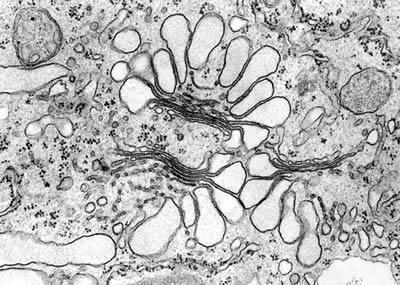
\includegraphics[width=0.6\textwidth]{sample_figure.png}
  \caption{TEM Image}
  \label{fig:tem}
\end{figure}

\subsection{Sub-Section Title}

\guidance{Please remove the texts in red which are given only as a guide.}

This page can be used as the sample for subsequent chapters. In the following the
Sub-Sections are also enumerated.

\subsection{Sub-Section Title}

This page can be used as the sample for subsequent chapters. In the following the
Sub-Sections are also enumerated.

\section{Section Title}

\subsection{Sub-Section Title}

This page can be used as the sample for subsequent chapters. In the following the
Sub-Sections are also enumerated.

In the following a Table is shown.

% ---- How to insert a table (caption goes ABOVE the table) ----
\begin{table}[H]
  \centering
  \caption{Measurements of Weather Conditions}
  \label{tab:weather}
  {\setstretch{1}
  \begin{tabular}{|c|c|c|c|c|c|}
    \hline
    Date & \begin{tabular}[c]{@{}c@{}}Temperature\\(maximum)\end{tabular}
         & \begin{tabular}[c]{@{}c@{}}Temperature\\(minimum)\end{tabular}
         & \begin{tabular}[c]{@{}c@{}}Humidity\\(maximum)\end{tabular}
         & \begin{tabular}[c]{@{}c@{}}Humidity\\(minimum)\end{tabular}
         & \begin{tabular}[c]{@{}c@{}}Wind Speed\\(average)\end{tabular} \\
    \hline
     & & & & & \\ \hline
     & & & & & \\ \hline
     & & & & & \\ \hline
  \end{tabular}\par}
\end{table}

\subsection{Sub-Section Title}

This page can be used as the sample for subsequent chapters. In the following the
Sub-Sections are also enumerated.

% =====================================================================
%  CHAPTER 5
% =====================================================================
\chapter{CONCLUSION AND FUTURE WORK}
\label{ch:conclusion}

\guidance{Summarize your key findings, contributions, limitations, and suggested directions
for future work here.}

% =====================================================================
%  REFERENCES  (IEEE style; APA is also allowed)
%  Your references live in the file  references.bib .
%  Cite them in the text with  \cite{key}  -- the list below is then
%  built and numbered automatically. See the Student Guide, Section 10.
% =====================================================================
\renewcommand{\HeadingAlign}{\raggedright}   % template: References/Appendix left-aligned

\renewcommand{\BibIntro}{%
  \guidance{Please remove the texts in red which are given only as a guide. The following
  is an example of writing the references which have been referenced to in the Thesis.
  Standard IEEE reference style should be used. Samples: [1] journal, [2] conference,
  [3] report, [4] book, [5] arXiv preprint, [6] webpage.
  If anyone wants, he/she can use APA style instead of IEEE style.}\par\medskip}
% ^ To remove this red note, delete everything between \renewcommand{\BibIntro}{ and }

% Sample references so the list is not empty. DELETE this line once you
% cite your own references with \cite{...}.
\nocite{zheng2018,oljira2017,cisco2019,goodfellow2016deep,devlin2018bert,pytorchdocs}

{\WordSpacing{1.5}
\bibliographystyle{IEEEtran}     % for APA write: \bibliographystyle{apalike}
\bibliography{references}       % = references.bib
\par}

% =====================================================================
%  APPENDIX
% =====================================================================
\chapter*{Appendix}
\addcontentsline{toc}{chapter}{Appendix}

\guidance{Add any supplementary material here: extra data, source code listings, survey
instruments, derivations, etc.}

\end{document}
